% !TeX root = ../main.tex

\chapter{相关理论与技术}

情感分析作为自然语言处理中的一项核心任务,旨在从文本或语音中自动识别出个体的情感状态。随着深度学习技术的兴起,情感分析已经从传统的规则和词典基础的方法,发展到更加依赖于机器学习和深度神经网络的复杂模型。这些进展使得情感分析在社交媒体监控、客户服务、心理健康评估等领域得到了广泛应用。与此同时,情感分析面临着大量挑战,例如情感表达的多样性、情绪标签的歧义性、以及情感信息的跨域迁移等问题。因此,研究高效且准确的情感分析方法对于推动智能化人机交互和情感计算具有重要意义。本章将对情感分析的相关理论与技术进行详细探讨,首先介绍情感分析中常见的预处理技术,然后深入分析在文本和语音情绪分析中应用广泛的深度学习技术。通过这些技术的研究,旨在为后续情感分析模型的设计和优化提供理论基础。

\section{预处理技术}

\subsection{文本预处理技术}

% 文本预处理是情感分析中的第一步,它的目的是将原始文本数据转化为机器学习模型可以处理的结构化数据。文本预处理的质量直接影响到后续分析的效果,因此它在自然语言处理(NLP)任务中扮演着至关重要的角色。通常,文本预处理包含多个步骤,例如文本清洗、去重、去停用词、分词等,每一步都在不同程度上提高了数据的质量和模型的性能。
在情感分析任务中,文本预处理作为基础性环节,旨在实现非结构化文本数据向机器学习模型可解析的规范化数据表示的转化。这一处理过程在自然语言处理(NLP)领域具有决定性影响,其执行质量显著制约着后续分析的有效性。典型的文本预处理流程由一系列标准化操作构成,包括但不限于文本清洗、数据去重、停用词过滤以及词汇切分等步骤,这些操作通过优化数据特征表示进而增强模型的泛化能力。


(1)文本清洗

文本清洗是文本预处理中的一个关键步骤,旨在去除文本中的噪音和不相关的信息,从而使得文本更加干净、规范。常见的清洗操作包括去除HTML标签、特殊字符、表情符号等非语言信息。这一步骤对于社交媒体数据和网络评论等非正式文本数据尤其重要,因为这些文本中可能包含大量的特殊符号、网页代码以及不适合分析的内容。此外,文本清洗还包括将文本中的多余空格、换行符进行处理,确保文本的格式一致。清洗后的文本可以帮助后续的情感分析模型减少噪声干扰,提高分析的准确性。

(2)去重方法

去重是文本预处理中不可忽视的步骤,尤其是在大规模文本数据集上进行分析时。由于数据集可能包含相同或重复的内容,去重操作可以减少冗余数据,避免模型因重复信息而出现过拟合的现象。去重方法通常基于文本相似度的度量,例如计算文本的Jaccard相似度或余弦相似度,进而确定哪些文本是重复的。对于一些高度重复的文本数据(如在线评论和论坛帖子),去重步骤能够有效地提高训练数据的多样性,增强模型的泛化能力。

(3)去停用词

停用词是指在情感分析过程中对情感判定没有实质性影响的常见词汇,如“的”、“是”、“在”等。虽然这些词在语法上起着重要作用,但在情感分析任务中,它们并不携带情感信息,反而可能会对情感分类造成干扰。因此,去停用词是文本预处理中的重要步骤。去停用词的方法一般通过预先定义的停用词列表进行过滤,或者基于语料的统计信息识别出频繁出现但不具有情感指示作用的词汇。通过去除这些无意义的词汇,情感分析模型能够集中精力分析更具情感信息的词汇,提高分析效率。需要注意的是,不同的任务和语境可能需要不同的停用词集合,去停用词的操作应根据实际情况灵活调整。

(4)分词技术

分词是将文本转化为可以进行后续处理的最小语义单元的过程。在文本处理中,分词通常是对句子或文本进行切分,将长篇的文字分割成较短的单元,如单词、短语或字符。对于中文文本,分词比英文文本更具挑战性,因为中文没有明显的单词分隔符。中文的分词任务常常依赖于词典、统计模型和深度学习模型等方法。英文文本的分词相对简单,通常是通过空格和标点符号来划分单词。然而,在一些复杂的场景中,如多义词、词组等,简单的基于空格的分词方法可能无法完全满足需求。为了提高分词的精度,近年来基于子词(subword)的分词技术,如 Byte-Pair Encoding(BPE) 和 SentencePiece 等,也在文本预处理中得到了广泛应用。这些方法能够有效地处理未登录词,并且在多语言情感分析中表现出较强的适应性。

\subsection{语音预处理技术}

语音预处理的目的是将原始语音信号转化为适合进行分析的特征,并在此过程中去除噪声和干扰信息,提高后续分析的准确性。语音预处理技术涵盖了多个步骤,如降噪、去除静音、特征提取等,这些步骤可以帮助消除录音中的背景噪音、强调语音的情感特征,并为模型输入提供更加清晰和有效的信息。以下是一些常见的语音预处理技术。

(1)降噪技术

降噪是语音预处理中非常关键的一步,尤其在实际应用中,语音信号往往会受到环境噪声的干扰。噪声可能来源于录音环境、背景人声、设备噪音等,这些噪声对语音情绪分析模型的性能产生负面影响。降噪的目的是通过滤波等技术去除这些不必要的噪音,并保留语音信号中的情感信息。常见的降噪方法包括谱减法、Wiener滤波、Kalman滤波等。谱减法通过估计噪声的频谱并从语音信号中减去该频谱来减少噪音,而Wiener滤波则基于噪声和语音信号的统计特性进行降噪。随着深度学习技术的发展,基于深度神经网络(DNN)和卷积神经网络(CNN)的降噪方法也逐渐得到应用,这些方法能够通过训练网络学习复杂的噪声特征并进行有效的噪声抑制,从而提高语音的质量。

(2)去除静音

在语音信号中,静音部分通常包含无用信息。尤其是在长时间的录音或对话过程中,静音区域可能会占据大量的时间,而这些部分对于情感分析任务的贡献较小。因此,去除静音部分是语音预处理中的一个常见步骤。去除静音的方法一般基于音频信号的幅度、能量或频谱特征来识别和去除静音段。常见的静音检测方法包括基于能量阈值的方法、基于自相关函数的方法以及基于机器学习的模型。基于能量阈值的方法通过计算每一帧的信号能量来判断该帧是否包含静音,而基于自相关函数的方法则通过分析信号的周期性来检测语音的持续性。随着深度学习技术的发展,基于RNN或LSTM的语音活动检测(VAD)技术也开始得到广泛应用,这些方法能够更精准地识别语音与静音的边界,并进行有效的去静音处理。

(3)特征提取

特征提取是语音预处理中的核心步骤,它将原始的语音信号转化为能够有效表示情感信息的特征。语音信号包含丰富的情感信息,但这些信息通常需要通过提取其特征来进行有效分析。常见的语音特征包括梅尔频率倒谱系数(MFCC)、线性预测倒谱系数(LPCC)、音高、能量、语速等。

梅尔频率倒谱系数(MFCC):MFCC是语音信号处理中最常用的特征之一,它通过模拟人耳对不同频率的敏感度,将语音信号的频谱信息转化为一组较为简洁的特征。MFCC能够有效捕捉语音的频谱特征,并对情感识别任务提供有效支持。

音高与基频(F0):音高是指声音的高低,通常与说话者的情绪状态密切相关。不同的情绪可能会导致音高的变化,因此音高也是情感识别中的一个重要特征。基频分析能够提供语音中频率的低频成分,是情感识别中常用的特征之一。

能量特征:语音信号的能量变化往往与情绪的强度和表达有关。例如,愤怒的语音通常伴随着较高的能量,而悲伤的语音则可能具有较低的能量。能量特征可以帮助模型识别语音的情感强度。

语速:语速也是语音情绪分析中的重要特征,快语速通常与兴奋、紧张等情绪相关,而慢语速则与冷静、抑郁等情绪相关。通过对语速的分析,模型可以有效区分不同的情感状态。

(4)音频分帧与窗口化

在处理长时间的语音信号时,通常需要将语音信号划分为多个短时间的帧进行分析。通过分帧处理,能够捕捉到语音信号的瞬时变化,避免长时间信号中的动态信息丧失。每一帧的信号通常通过加窗(如Hamming窗或Hanning窗)来减少边缘效应,使得语音信号在每一帧内的频谱特征更加平滑,进而提高特征提取的准确性。

\section{Tokenizer 分词技术}

% 分词(Tokenization)是将连续的文本转换为基本单位(如单词、子词或字符)的过程。分词的质量直接影响到后续文本处理的效果。根据分词的粒度和方式,分词技术可以大致分为基于单词的分词、基于子词的分词等。不同语言的分词方法有所不同,尤其在英文和中文的处理上具有较大差异。下面将详细介绍基于单词的分词技术,以及基于子词的分词技术。

在自然语言处理领域,文本分词(Tokenization)是指将连续文本序列转化为离散语言单元(包括单词、子词或字符)的关键预处理步骤。该技术的处理效果会显著制约下游文本分析任务的性能表现。依据处理粒度的不同,现有分词方法主要划分为单词级分词和子词级分词两大类别。需要特别注意的是,不同语系的分词处理存在显著区别,尤其在英语和汉语这两种典型语言中体现得最为明显。本文后续将系统阐述单词级分词技术和子词级分词技术的具体实现方法。

\subsection{基于单词的分词}

基于单词的分词技术是将句子按空格、标点符号等分割成一个个单词(Token),这一方法较为直接,适用于以空格作为单词分隔符的语言,如英语等。然而,中文等语言则没有空格,分词任务因此变得更加复杂。

在英文中,基于单词的分词方法非常直接,通常通过空格、标点符号和其他分隔符来将句子划分为一个个单词。英文单词分词的典型步骤包括:首先找到句子中的空格,随后根据空格将句子拆分成多个单词。标点符号(如句号、逗号等)通常被视为与单词分离的标记,并被单独提取出来。例如,给定句子:"I love natural language processing.",基于空格和标点的单词分词结果如图~\ref{word-based-english} 所示。在这个例子中,单词 "I"、"love"、"natural"、"language"、"processing" 和句号 "." 被分开作为不同的 Token。对于英文,除了基本的空格分隔外,还可以利用更复杂的规则来处理一些特殊情况,比如将合成词(如 "don't"、"I'm")处理成其子组成部分(如 "do" 和 "n't",或 "I" 和 "'m")。

\begin{figure}[ht]
  \centering
  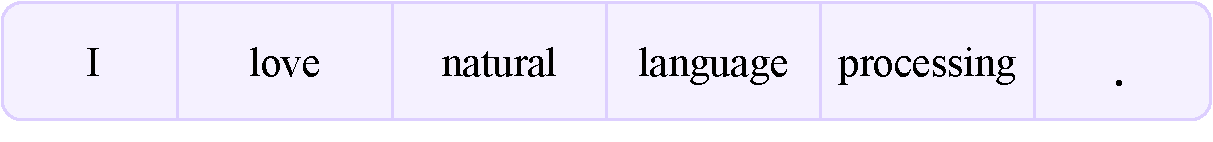
\includegraphics[width=0.7\textwidth]{word-based-english.pdf}
  \caption{基于单词的英文分词示例}
  \label{word-based-english}
\end{figure}

与英文不同,中文文本没有空格作为单词分隔符,因此中文的分词问题相对复杂。在中文中,一个词通常由多个汉字组成,分词任务的目标是将一段连续的汉字序列切分为有意义的词汇单元。例如,给定中文句子:"我喜欢自然语言处理",本文要将其拆分成合适的单词(Token)。使用基于单词的分词方法,结果如图~\ref{word-based-chinese} 所示。在这个例子中,中文分词通过识别词语之间的语义关联将句子切分成了几个有意义的词汇单位,如 "我"、"喜欢"、"自然"、"语言" 和 "处理"。中文分词通常依赖于词典和统计方法。基于词典的分词方法通过查找词典中的词语来决定分词位置。统计分词方法则通过计算词频和概率,结合上下文信息,来判断哪些字符序列应当作为一个单词。因此,中文分词不仅需要处理语言结构的特点,还需要解决多义词、歧义分词等问题。

\begin{figure}[ht]
  \centering
  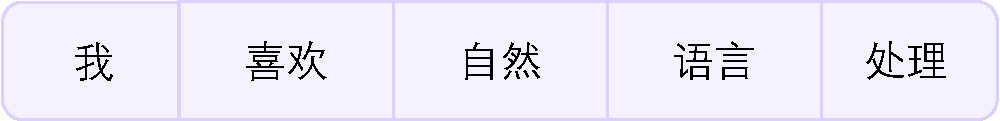
\includegraphics[width=0.7\textwidth]{word-based-chinese.pdf}
  \caption{基于单词的中文分词示例}
  \label{word-based-chinese}
\end{figure}

\subsection{基于子词的分词}

基于子词的分词方法已成为处理自然语言文本的一种重要手段,特别是在处理词汇外词(OOV,Out-of-Vocabulary)时表现尤为突出。传统的基于单词的分词方法对一些不常见的词语处理能力较弱,特别是对于未登录词或低频词,常常无法有效地进行分词。为了解决这一问题,基于子词的分词方法逐渐被提出,并得到广泛应用。基于子词的分词方法通过将单词拆分为更小的单位(如子词或字形)来进行处理,从而在词汇稀缺的情况下仍能保证较好的性能。常见的基于子词的分词方法包括 Byte-Pair Encoding(BPE) 和 SentencePiece。这两种方法通过学习字与字之间的频率关系,将文本拆分为更细粒度的单元,从而克服了传统单词分词方法的不足。

Byte-Pair Encoding(BPE)最初是用于文本压缩的技术,但它也很自然地被引入到自然语言处理中,作为一种有效的分词方法。BPE的基本思想是,通过合并频率最高的字符对来构建词汇表,并反复执行这一过程直到达到预定的词汇量。BPE主要通过三个步骤进行工作:(1)BPE 将文本中的每个单词拆解为字符,并计算所有字符对(即连续字符的组合)在文本中的出现频率,例如,考虑单词 "low" 和 "lower",拆分为字符;(2)BPE计算字符对的频率,最常见的字符对会被合并为一个新的符号,假设 "l o" 的频率最高,就会将它们合并为 "lo",得到新的词汇单元;(3)重复这一过程,每次选择出现频率最高的字符对进行合并,直到达到所需的词汇表大小。BPE 的优势在于它通过递归地合并字符对,能够有效地处理不常见的单词和词汇外问题。例如,对于低频词 "unhappiness",BPE可以将其拆分为更小的单位,如 "un", "happiness" 或 "un", "hap", "pi", "ness",从而使模型能够处理这些不常见的词汇。BPE的具体合并过程可以表示为以下公式:
\begin{equation}
    P_{\text{BPE}}(w) = \arg\max_{(v_i, v_j) \in V} \text{count}(v_i, v_j),
\end{equation}
其中,$V$ 是当前的词汇表,$\text{count}(v_i, v_j)$ 表示字符对 $(v_i, v_j)$ 的频率,BPE通过合并最高频率的字符对来更新词汇表。

\subsubsection{SentencePiece 方法}

SentencePiece 是 Google 提出的另一种基于子词的分词方法,它通过无监督学习从原始文本中直接生成子词单元。与BPE方法不同,SentencePiece 并不依赖于预先设定的词典,而是基于字符的频率信息自动生成一个新的词汇表。SentencePiece的核心思想是通过统计学方法从原始文本数据中学习一个最优的词汇表示,处理每一个字符序列的最大似然估计,进而生成子词单元。SentencePiece 的工作流程包括两个步骤:(1)给定一个原始文本数据集,SentencePiece将其转换为一个字符序列(包括所有的字符和符号);(2)SentencePiece 使用一个基于概率的模型,通过最大化似然函数来训练一个子词词汇表,这个模型的目标是将输入的字符序列映射到一个固定大小的子词单元集合中,使得原始文本能够高效地通过这些子词表示出来。

在 SentencePiece 模型中,输入文本数据经过预处理后,首先会被拆解成单一的字符单元。接着,模型通过迭代的方式,从这些字符中学习频繁出现的字母对、字符组合等,并不断合并它们形成新的子词单元。这个过程中,SentencePiece采用的是一种基于最大似然估计的方法,来选择那些出现频率较高的字符组合进行合并。与BPE不同,SentencePiece不依赖空格或其他标点符号来划分单词,而是直接在字符层面进行操作。它的一个主要优势是能够处理所有语言,包括没有明确单词分隔符的语言(如中文、日语等)。例如,中文文本“我喜欢学习”会被直接拆解为子词单位,如“我”,“喜欢”,“学习”。这使得SentencePiece在多种语言的分词任务中都表现出色。数学上,SentencePiece的目标是最大化以下似然函数:
\begin{equation}
    L = \prod_{t=1}^{T} P(w_t | \theta),
\end{equation}
其中,$w_t$ 是文本中第$t$个词,$\theta$ 是模型参数。通过最大化该似然函数,SentencePiece模型能够找到一个最佳的子词表示,自动生成词汇表并进行有效的分词。

\section{深度学习情绪分析技术}


% 深度学习模型能够自动从数据中提取复杂的特征,避免了人工特征设计的繁琐过程,极大提升了情感分析任务的准确性和泛化能力。本节将介绍几种常见的深度学习情感分析技术,包括卷积神经网络(CNN)、循环神经网络(RNN)、预训练文本模型(如BERT、GPT和LLaMA),以及在语音情绪分析中应用的预训练语音模型(如HuBERT和WavLM)。

在情感分析领域,基于深度学习的解决方案通过表征学习的自动化机制,显著降低了传统方法中人工设计特征的主观性和复杂性。这种数据驱动的建模范式不仅增强了分类性能,还提高了模型在不同场景下的适应能力。本部分将系统梳理当前主流的深度情感分析架构,首先讨论面向文本数据的神经网络模型,涵盖卷积结构、循环网络以及基于Transformer的大规模预训练语言模型;其次阐述针对语音信号的情感识别系统,重点分析自监督预训练音频表征的最新进展。

\subsection{卷积神经网络}

% 卷积神经网络(CNN)最早被提出用于图像识别,但其强大的特征提取能力使其同样适用于自然语言处理(NLP)任务,尤其在情感分析中取得了显著的成功。CNN的优势在于能够自动学习数据中的局部特征和模式,从而在处理文本数据时具有很好的表现。如图 ~\ref{textcnn} 所示,以 TextCNN 为例,在情感分析任务中,TextCNN的基本原理是通过卷积操作提取输入文本中的局部特征,这些特征通常与情感相关的词组、短语或者情感表达方式相关。通过对文本进行词嵌入(word embedding)表示后,应用卷积核(filters)来识别文本中的局部结构。例如,卷积核可以学习到“非常喜欢”这种组合词的情感特征。

在计算机视觉领域首次引入的卷积神经网络(CNN),凭借其卓越的特征学习能力,现已广泛应用于自然语言处理领域,特别是在情感分类任务中展现出优异性能。该模型的核心价值在于其无需人工干预即可从数据中捕获局部模式和关键特征,这一特性使其在文本分析任务中表现突出。以TextCNN架构为例(见图~\ref{textcnn}),该模型首先将输入文本转换为分布式表示,随后利用多个卷积核对文本的局部语义单元进行特征提取,这些单元往往与情感表达密切关联。具体而言,模型能够自动识别如"非常喜欢"等具有情感倾向的词语组合。

\begin{figure}[ht]
  \centering
  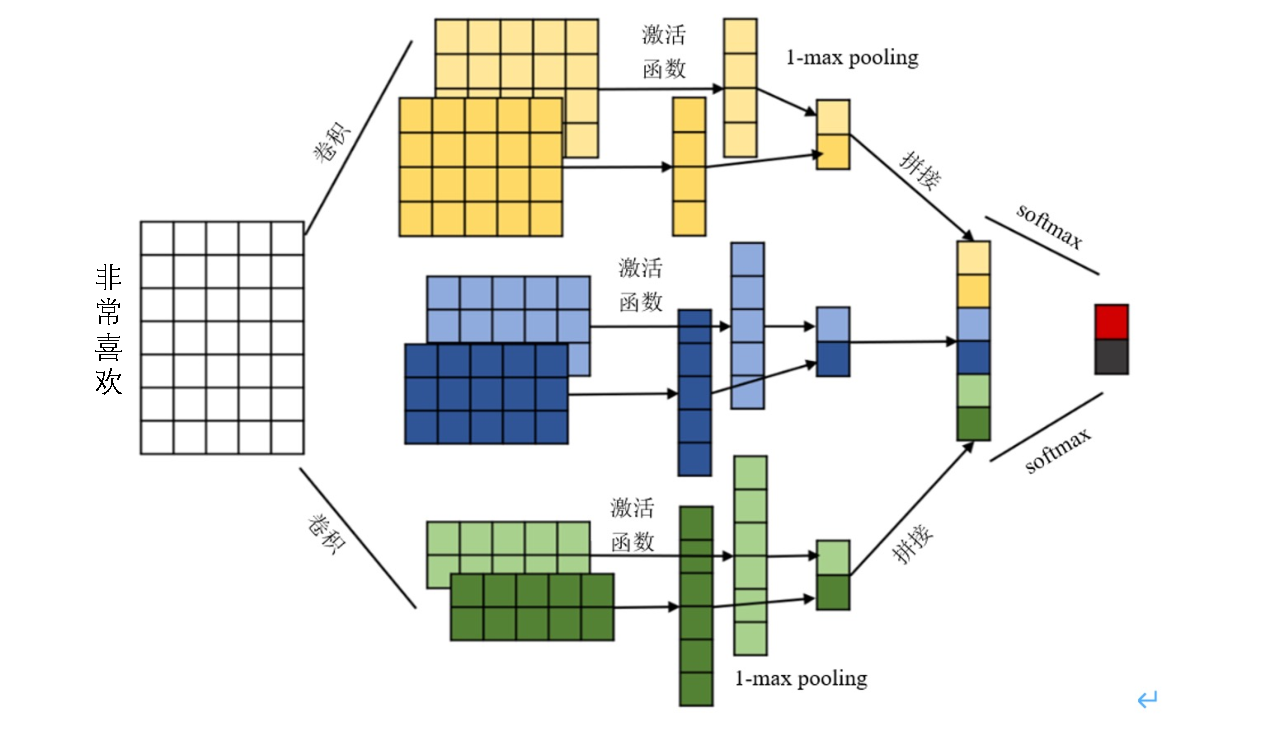
\includegraphics[width=0.7\textwidth]{textcnn.pdf}
  \caption{TextCNN 模型示意图}
  \label{textcnn}
\end{figure}

% 文本通过词嵌入层转化为词向量后,卷积操作通过滑动窗口的方式在词向量矩阵上进行卷积,提取出句子中包含情感信息的局部特征。接着,池化层(pooling layer)通过下采样进一步减少维度和计算量,保留最重要的特征信息。最后,经过全连接层(fully connected layer),输出情感分类的结果(如积极、消极、中立等)。CNN的优势在于它能够捕捉到文本中的局部依赖关系,因此在处理情感短语、情感词对等方面具有较好的表现。

经过词向量转换的文本数据,通过卷积核的滑动扫描操作,可有效抽取出蕴含情感信息的语义片段。随后,降采样层对特征进行压缩处理,在降低计算复杂度的同时保留最具判别性的特征。最终,分类层根据提取的特征完成情感极性预测(如正面、负面或中性)。这种架构的突出优势在于其对文本局部语义关联的捕捉能力,使其在处理情感修饰词对和情感表达短语时具有独特优势。

\subsection{循环神经网络}

% 循环神经网络(RNN)是一类特别适合处理序列数据的神经网络,尤其适用于文本数据的处理。如图 ~\ref{rnn} 所示,与CNN不同,RNN的特点在于它能够捕捉序列中元素之间的时序依赖关系。RNN能够处理文本中的上下文信息,通过逐词输入的方式处理句子,学习到文本中的时间依赖性。在情感分析任务中,RNN可以逐步分析句子中的每个单词,并更新隐藏状态(hidden state),从而捕捉到情感的变化。例如,在情感分析任务中,RNN能够根据上下文信息判断情感的流向,能够较好地处理多轮对话或长文本的情感分析任务。

作为一类专门建模时序信息的神经网络架构,循环神经网络(RNN)尤其擅长文本数据的分析与处理。区别于卷积神经网络(CNN),RNN的核心优势在于其能够有效建模序列元素间的动态关联性(如图~\ref{rnn}所示)。通过迭代式输入,该网络能学习文本的时间依赖性并构建上下文表征。在情感分析领域,RNN通过逐步解析语句中的词汇并动态更新隐含表征,从而准确识别情感倾向变化,这种特性使其在多轮对话或长文本分析中表现优异。

\begin{figure}[ht]
  \centering
  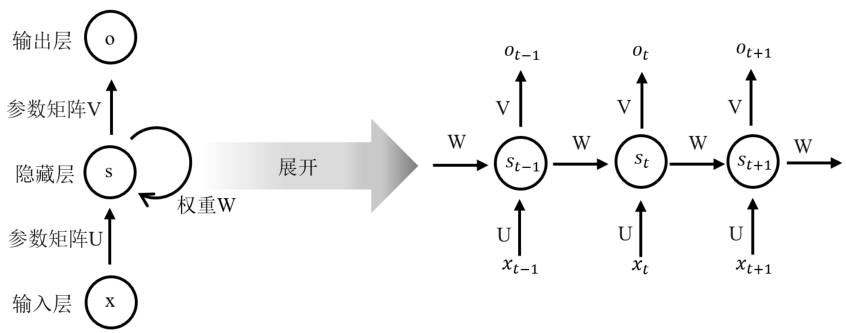
\includegraphics[width=0.7\textwidth]{rnn.pdf}
  \caption{RNN 模型示意图}
  \label{rnn}
\end{figure}

% 传统的RNN模型存在梯度消失和梯度爆炸的问题,因此,长短期记忆网络(LSTM)和门控循环单元(GRU)等变种被提出并广泛应用于情感分析任务。LSTM通过引入三个门控机制(输入门、遗忘门、输出门)来控制信息的流动,使得网络能够在长序列中捕捉长程依赖关系,避免了传统RNN的梯度消失问题。GRU则是LSTM的一种简化形式,具有相似的性能,但计算量较少。

然而,基础 RNN 存在梯度消失与梯度爆炸的固有缺陷。为此,研究者提出了长短期记忆网络(LSTM)和门控循环单元(GRU)等改进架构。LSTM设计了输入门、遗忘门与输出门三类调控单元,通过精细化信息流管理实现长程依赖建模,有效解决了梯度异常问题。GRU作为LSTM的轻量化版本,通过精简结构降低了计算复杂度,同时保持了相近的建模能力。

\subsection{预训练文本模型}

% 预训练模型通过在大规模语料库上进行预训练,能够学习到语言的丰富表示,并在此基础上进行微调,适应特定的任务。以下将介绍三种主要的预训练文本模型:BERT、GPT和LLaMA。

近年来,基于海量文本数据的自监督学习技术显著提升了自然语言处理模型的性能。通过在大规模无标注语料上进行预训练,这些模型能够获取深层次的语言特征表示,随后可通过迁移学习策略适配各类下游应用。本文重点探讨三种具有代表性的文本预训练架构:BERT、GPT及LLaMA。

\begin{figure}[ht]
  \centering
  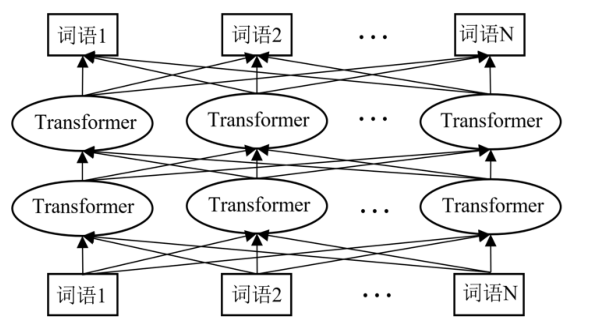
\includegraphics[width=1\textwidth]{BERT.pdf}
  \caption{BERT 模型示意图}
  \label{bert}
\end{figure}

(1)基于双向编码器的BERT模型

由Google研发的BERT(Bidirectional Encoder Representations from Transformers)\cite{Devlin_Chang_Lee_Toutanova_2019}创新性地采用了Transformer编码器堆叠结构,通过双向上下文建模机制显著提升了语义表征质量。如图\ref{bert}所示,该模型突破了传统单向语言模型的局限,实现了基于全局上下文信息的动态词向量生成。在情感识别领域,BERT首先在BookCorpus等大规模语料完成预训练,建立对语言系统的深层认知,继而通过参数微调实现特定情感分类任务。其创新性体现在两方面:首先设计了遮蔽语言建模任务(MLM),通过预测被遮蔽的词汇单元来强化上下文理解;其次引入句子关系预测任务(NSP),增强模型对语句间逻辑关联的把握能力。

(2)基于自回归解码器的 GPT 模型

OpenAI提出的GPT(Generative Pretrained Transformer)\cite{Radford_Narasimhan_Salimans_Sutskever}系列采用Transformer解码器结构,通过自左向右的自回归方式构建语言模型。这种单向建模特性使其特别适合文本生成类应用。在情感分析任务中,GPT首先通过海量文本预训练掌握语言生成规律,再通过监督微调优化情感判别性能。相较于判别式模型,其核心优势在于能够通过概率生成方式重构情感语义,这种特性使其在对话系统、创意写作等场景表现突出。随着GPT-3等后续版本的演进,模型参数量级和生成质量持续突破,为情感计算等NLP任务提供了更强大的基础支撑。

(3)LLaMA 模型

Meta公司发布的LLaMA(Large Language Model Meta AI)\cite{Touvron_Lavril_Izacard_Martinet_Lachaux_Lacroix_Roziere_Goyal_Hambro_Azhar_et}系列致力于构建高性价比的开源语言模型。该架构通过对公开语料的高效训练,在保持优异性能的同时显著降低计算资源消耗。在情感理解方面,LLaMA展现出对复合情感和隐含情感的出色解析能力。其技术特色在于通过精心的参数设计和数据筛选策略,在模型效率与准确性之间实现了优化平衡,为资源受限场景下的情感分析应用提供了新的解决方案。

\subsection{预训练语音模型}

在语音情绪分析中,预训练语音模型近年来也取得了长足进展。包括两种常见的预训练语音模型:HuBERT\cite{Hsu_Bolte_Tsai_Lakhotia_Salakhutdinov_Mohamed_2021} 和 WavLM\cite{Chen_2022}。

HuBERT(Hidden-Unit BERT)是Facebook提出的一种自监督学习语音表示学习方法。该方法将语音信号转化为一系列隐含单元(hidden units),并利用这些单元进行上下文建模。通过自监督学习,HuBERT模型可以在大规模无标签语音数据上进行训练,学习到语音的深层表示,进而用于下游的语音任务,如语音情绪分析。

WavLM(Waveform-based Language Model)是 Microsoft 提出的一种基于波形的自监督学习语音模型。WavLM直接对原始音频波形进行建模,通过自监督学习来学习语音信号中的有用特征。与传统的语音处理方法不同,WavLM不依赖于手工提取的特征,而是通过深度神经网络直接从原始音频中学习特征,从而为语音情绪分析任务提供了更强的能力。WavLM的自监督学习框架使得它在语音情感识别中能够取得很好的效果,尤其在处理复杂的语音情感变化时,能够从音频中提取出更加丰富的情感信息。

\section{本章小节}

本章介绍了情感分析的相关技术,包括文本和语音的预处理方法、Tokenizer分词技术及深度学习模型的应用。重点讨论了文本清洗、去重、去停用词、分词,以及语音降噪和特征提取等预处理步骤,它们为情感分析提供了有效的数据输入。分词技术部分介绍了基于单词和子词的分词方法,特别是Byte-Pair Encoding(BPE)和SentencePiece的应用。接着,分析了卷积神经网络(CNN)、循环神经网络(RNN)以及预训练文本模型(如BERT、GPT、LLaMA)在情感分析中的优势,并探讨了预训练语音模型(如HuBERT、WavLM)在语音情绪分析中的重要作用。预训练模型为情感分析提供了强大的数据表示能力,并将在后续的研究中用于进一步提升模型的性能。
